\documentclass{beamer}

\newcommand{\course}{CS 1331 Introduction to Object Oriented Programming}
\newcommand{\lesson}{Swing, Part 3}
\newcommand{\code}{http://www.cc.gatech.edu/~simpkins/teaching/gatech/cs1331/code}

\author[Chris Simpkins]
{Christopher Simpkins \\\texttt{chris.simpkins@gatech.edu}}
\institute[Georgia Tech] % (optional, but mostly needed)

\date[CS 1331]{}


\newcommand{\course}{Introduction to Object-Oriented Programming}
\subject{\course}
\title[\lesson]{\course}
\subtitle{\lesson}

\author[CS 1331]
{Christopher Simpkins \\\texttt{chris.simpkins@gatech.edu}}
\institute[Georgia Tech]

\date[]{}

\newcommand{\link}[2]{\href{#1}{\textcolor{blue}{\underline{#2}}}}
\newcommand{\code}{http://www.cs1331.org/code}

\usepackage{colortbl}

% If you have a file called "university-logo-filename.xxx", where xxx
% is a graphic format that can be processed by latex or pdflatex,
% resp., then you can add a logo as follows:

% \pgfdeclareimage[width=0.6in]{coc-logo}{cc_2012_logo}
% \logo{\pgfuseimage{coc-logo}}

\mode<presentation>
{
  \usetheme{Berlin}
  \useoutertheme{infolines}

  % or ...

 \setbeamercovered{transparent}
  % or whatever (possibly just delete it)
}

\usepackage{tikz}
% Optional PGF libraries
\usepackage{pgflibraryarrows}
\usepackage{pgflibrarysnakes}
\usepackage{pgfplots}
\usepackage{fancybox}
\usepackage{listings}
\usepackage{hyperref}
\hypersetup{colorlinks=true,urlcolor=blue}
\usepackage[english]{babel}
% or whatever

\usepackage[latin1]{inputenc}
% or whatever

\usepackage{times}
\usepackage[T1]{fontenc}
% Or whatever. Note that the encoding and the font should match. If T1
% does not look nice, try deleting the line with the fontenc.


\usepackage{listings}

% "define" Scala
\lstdefinelanguage{scala}{
  morekeywords={abstract,case,catch,class,def,%
    do,else,extends,false,final,finally,%
    for,if,implicit,import,match,mixin,%
    new,null,object,override,package,%
    private,protected,requires,return,sealed,%
    super,this,throw,trait,true,try,%
    type,val,var,while,with,yield},
  otherkeywords={=>,<-,<\%,<:,>:,\#,@},
  sensitive=true,
  morecomment=[l]{//},
  morecomment=[n]{/*}{*/},
  morestring=[b]",
  morestring=[b]',
  morestring=[b]""",
}

\usepackage{color}
\definecolor{dkgreen}{rgb}{0,0.6,0}
\definecolor{gray}{rgb}{0.5,0.5,0.5}
\definecolor{mauve}{rgb}{0.58,0,0.82}

% Default settings for code listings
\lstset{frame=tb,
  language=scala,
  aboveskip=2mm,
  belowskip=2mm,
  showstringspaces=false,
  columns=flexible,
  basicstyle={\scriptsize\ttfamily},
  numbers=none,
  numberstyle=\tiny\color{gray},
  keywordstyle=\color{blue},
  commentstyle=\color{dkgreen},
  stringstyle=\color{mauve},
  frame=single,
  breaklines=true,
  breakatwhitespace=true,
  keepspaces=true
  %tabsize=3
}


% If you wish to uncover everything in a step-wise fashion, uncomment
% the following command:

% \beamerdefaultoverlayspecification{<+->}


\begin{document}

\begin{frame}
  \titlepage
\end{frame}

%------------------------------------------------------------------------
\begin{frame}[fragile]{Java Projects}

Today's example will involve many classes, so we'll begin by learning how to organize a multi-file (and multi-library) Java project
\begin{itemize}
  \item the classpath and third-party libraries
  \item separating source and compiler output
  \item project directory layout
  \item packages
\end{itemize}

\end{frame}
%------------------------------------------------------------------------

%------------------------------------------------------------------------
\begin{frame}[fragile]{The Classpath}


Just as your operating system shell looks in the {\tt PATH} environment variable for executable files, JDK tools (such as {\tt javac} and {\tt java}) look in the {\tt CLASSPATH} for Java classes. To specify a classpath:

\begin{itemize}
\item set an environment variable named {\tt CLASSAPTH}, or
\item specify a classpath on a per-application basis by using the {\tt -cp} switch.  The classpath set with {\tt -cp} overrides the {\tt CLASSPATH} environment variable.
\end{itemize}
Pro tip: don't use the {\tt CLASSPATH} environment variable.  If it's already set, clear it with (on Windows):
\begin{lstlisting}[language=Java]
C:> set CLASSPATH=
\end{lstlisting}
or (on Unix):
\begin{lstlisting}[language=Java]
$ unset CLASSPATH
\end{lstlisting}

\end{frame}
%------------------------------------------------------------------------

%------------------------------------------------------------------------
\begin{frame}[fragile]{Classpath Elements}

\vspace{-.05in}
A classpath specification is a list of places to find {\tt .class} files and other resources.  Two kinds of elements in this list:
\vspace{-.05in}
\begin{itemize}
\item directories in which to find {\tt .class} files on the filesystem, or
\item {\tt .jar} files that contain archives of directory trees.
\end{itemize}

A {\bf J}ava {\bf ar}chive, or jar file, is a Zip-formatted archive of a directory tree containing {\tt .class} files and other files.
\vspace{-.05in}
\begin{itemize}
\item To create a JAR file: {\tt jar cf jar-file input-file(s)}
\item To view the contents of a JAR file {\tt jar tf jar-file}
\item To extract the contents of a JAR file: {\tt jar xf jar-file} or {\tt unzip jar-file}
\item To extract specific files from a JAR file: {\tt jar xf jar-file archived-file(s)}
\item To run an application packaged as a JAR file (requires the Main-class manifest header): {\tt java -jar app.jar}
\end{itemize}
See
\link{http://docs.oracle.com/javase/tutorial/deployment/jar/index.html}{http://docs.oracle.com/javase/tutorial/deployment/jar/index.html} for more on jar files.

\end{frame}
%------------------------------------------------------------------------

%------------------------------------------------------------------------
\begin{frame}[fragile]{Specifying a Classpath}


To compile and run a program with compiler output ({\tt .class} files) in the current directory and a library Jar file in the {\tt lib} directory called {\tt util.jar}, you'd specify the classpath like this:
\vspace{-.05in}
\begin{lstlisting}[language=bash]
$ ls -R # -R means recursive (show subdirectory listings)
MyProgram.java     AnotherClass.java

./lib:
util.jar
$ javac -cp .:lib/util.jar *.java # : separates classpath elements
$ java -cp .:lib/util.jar MyProgram # would be ; on Windows
\end{lstlisting}

Notice that you include the entire classpath in the {\tt -cp}, which includes the current directory ({\tt .} means ``current directory'').

\end{frame}
%------------------------------------------------------------------------

%------------------------------------------------------------------------
\begin{frame}[fragile]{Separating Source and Compiler Output}


To reduce clutter, you can compile classes to another directory with {\tt -d} option to {\tt javac}
\begin{lstlisting}[language=Java]
$ mkdir target
$ javac -d target HelloWorld.java
$ ls target/
HelloWorld.class
\end{lstlisting}
Specify classpath for an application with the {\tt -cp} option to {\tt
  java}.
\begin{lstlisting}[language=Java]
$ java -cp ./target HelloWorld
Hello, world!
\end{lstlisting}

If you really want to keep your project's root directory clean (and you do), you can put your source code in another directory too, like {\tt src}.
\begin{lstlisting}[language=Java]
$ mkdir src
$ mv HelloWorld.java src/
$ javac -d ./target src/HelloWorld.java
$ java -cp ./target HelloWorld
Hello, world!
\end{lstlisting}

\end{frame}
%------------------------------------------------------------------------

%------------------------------------------------------------------------
\begin{frame}[fragile]{Project Directory Layout}


Source Directories
\begin{itemize}
\item {\tt src/} for Java source files
\item {\tt src/resources/} for resources that will go on the classpath, like image files
\end{itemize}

Third Party Libraries
\begin{itemize}
\item {\tt lib/} for jar files
\end{itemize}


Output Directories
\begin{itemize}
\item {\tt target/} for compiled Java .class files and resources copied from {\tt src/resources/}
\end{itemize}

We'll use this simple layout, but the de-facto standard Java project directory layout for "professional" Java projects introduced by the Maven build tool can be found at \link{http://maven.apache.org/guides/introduction/introduction-to-the-standard-directory-layout.html}{http://maven.apache.org/guides/introduction/introduction-to-the-standard-directory-layout.html}

\end{frame}
%------------------------------------------------------------------------

%------------------------------------------------------------------------
\begin{frame}[fragile]{Organizing your Code in Packages}


All professional Java projects organize their code in packages.  The standard package naming scheme is to use reverse domain name, followed by project specific packages.  For our CompanyGUI application we could use the package name
\vspace{-.05in}
\begin{lstlisting}[language=Java]
package edu.gatech.cs1331.companygui;
\end{lstlisting}
and source files would be located in a directory under your {\tt src/} directory as follows
\begin{lstlisting}[language=Java]
src/edu/gatech/cs1331/companygui/
\end{lstlisting}
\vspace{-.05in}
And if you tell {\tt javac} to put compiler output in {\tt target/} then the compiled {\tt .class} file would end up in:
\begin{lstlisting}[language=Java]
target/edu/gatech/cs1331/companygui/
\end{lstlisting}
\vspace{-.05in}
Aside from organization, packages ensure that names are unique.  Using reverse domain names leverages the fact that internet domain names are non-ambiguous.

\end{frame}
%------------------------------------------------------------------------

%------------------------------------------------------------------------
\begin{frame}[fragile]{Swing Applications}


\begin{itemize}
\item Inner classes
\item Built-in dialogs
\item Lists, ListModels and the MVC Pattern
\item General Structure of Swing Hierarchy
\item ScrollPanes and the Decorator Pattern
\item Custom Dialog Boxes
\end{itemize}

We'll cover a lot today.  Think of today's lecture as a guided tour through an example Swing application, \link{\code/swing/companygui}{Company GUI}, which provides a GUI for the company classes we wrote a few weeks ago.  After the tour you can look at this application for examples to guide your own Swing app development.

\end{frame}
%------------------------------------------------------------------------

%------------------------------------------------------------------------
\begin{frame}[fragile]{Inner Classes}


We've defined our listeners as public top-level classes, but if they're only used in one class they can be defined within the class that uses them:

\begin{lstlisting}[language=Java]
public class CompanyFrame extends JFrame {

    private class NewEmpListener implements ActionListener {
        public void actionPerformed(ActionEvent e) { ... }
    }
// ...
\end{lstlisting}

And instantiated where needed:

\begin{lstlisting}[language=Java]
JButton newEmpButton = new JButton("New Employee...");
newEmpButton.addActionListener(new NewEmpListener());
\end{lstlisting}


\end{frame}
%------------------------------------------------------------------------

%------------------------------------------------------------------------
\begin{frame}[fragile]{Anonymous Inner Classes}


If an inner class is used only once, we can define it and instantiate an instance of it anonymously at the same time:
\begin{lstlisting}[language=Java]
newEmpButton.addActionListener(new ActionListener() {
    public void actionPerformed(ActionEvent e) {
        System.out.println("New button.  It was clicked.");
    }
});
\end{lstlisting}

\begin{itemize}
\item The syntax {\tt new ActionListener() \{ ... \}} means ``instantiate an instance of a class that's a subclass of {\tt ActionListener}'.'
\item Required method definitions are given between {\tt \{ ... \}}.
\end{itemize}

You'll see this idiom a lot in Swing code.


\end{frame}
%------------------------------------------------------------------------

%------------------------------------------------------------------------
\begin{frame}[fragile]{Dialog Windows}


A dialog window:
\begin{itemize}
\item is an independent subwindow that conveys information or gets input form the user.
\item can be {\it modal}, meaning that the dialog window blocks its parent {\tt Frame} while the dialog is visible, or {\it modeless} meaning it does not block its parent window.
\end{itemize}
In Swing:
\begin{itemize}
\item Every dialog is dependent on a Frame.  When a dialog's parent Frame is destroyed, so is the dialog.
\item Simple modal dialogs can be created easily with {\tt JOptionPane}.
\item Custom dialogs can be created by extending {\tt JDialog}.
\end{itemize}

\end{frame}
%------------------------------------------------------------------------

%------------------------------------------------------------------------
\begin{frame}[fragile]{Simple Dialogs with {\tt JOptionPane}}


{\tt JOptionPane} has several static methods that instantiate and display simple dialogs.  The most common are (from the Java API):

\begin{itemize}
\item {\tt showConfirmDialog} asks a confirming question, like yes/no/cancel.
\item {\tt showInputDialog} prompts prompts the user for input.
\item {\tt showMessageDialog} displays a message to the user.
\item {\tt showOptionDialog} is The Grand Unification of the above three.
\end{itemize}
For example, the line:
\begin{lstlisting}[language=Java]
JOptionPane.showMessageDialog(null, "Simple message.");
\end{lstlisting}
\begin{columns}[c]
\begin{column}{2in}
displays the dialog:
\end{column}
\begin{column}{2in}
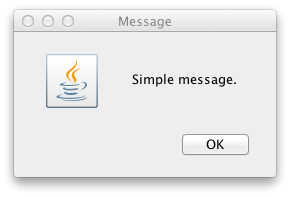
\includegraphics[height=1in]{simple-message-dialog.png}
\end{column}
\end{columns}

\end{frame}
%------------------------------------------------------------------------

%------------------------------------------------------------------------
\begin{frame}[fragile]{{\tt JFileChooser}}

Swing provides dialog windows for common tasks like choosing colors and choosing files.  Here's a general pattern for using {\tt JFileChooser}:
\begin{lstlisting}[language=Java]
  // This is how you get the present working directory
  File thisDir = new File(System.getProperty("user.dir"));
  // Pass thisDir to JFileChooser's constructor to open
  // the JFileChooser in the present working directory
  JFileChooser chooser = new JFileChooser(thisDir);
  // showOpenDialog() blocks until the user clicks ``OK'' or ``Cancel''
  int returnVal = chooser.showOpenDialog(null);
  // The return value from showOpenDialog() tells you how the user
  // dismissed the dialog
  if (returnVal == JFileChooser.APPROVE_OPTION) {
      File file = chooser.getSelectedFile();
      // do somethign with file ...
  }
\end{lstlisting}

See \link{\code/swing/companygui/src/edu/gatech/cs1331/companygui/CompanyGui.java}{CompanyGui.java} for an example.


\end{frame}
%------------------------------------------------------------------------

%------------------------------------------------------------------------
\begin{frame}[fragile]{General Structure of Swing Programs}

Typically a Swgin GUI program will have
\begin{itemize}
\item a ``main'' class (often in {\tt Main.java}) that is responsible for handling command line arguments (if any), initializing the application configuration (perhaps form a properties file), and opening the application's main frame
\item a ``main frame'' that represents the application's main GUI component, it's ``top level'' or ``home screen.''
\end{itemize}

In the \link{\code/swing/companygui}{Company GUI} example \link{\code/swing/companygui/src/edu/gatech/cs1331/companygui/CompanyGui.java}{CompanyGui.java} is the main class and \link{\code/swing/companygui/src/edu/gatech/cs1331/companygui/CompanyFrame.java}{CompanyFrame.java} is the main frame.


\end{frame}
%------------------------------------------------------------------------


%------------------------------------------------------------------------
\begin{frame}[fragile]{The Model-View-Controller Design Pattern}
\vspace{-.1in}
\begin{center}
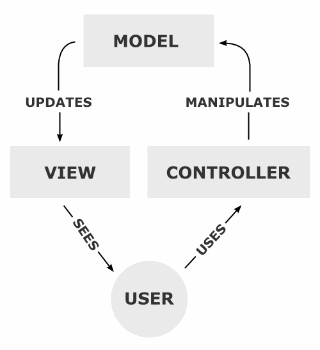
\includegraphics[height=1.5in]{MVC-Process.png}\footnote{\url{http://en.wikipedia.org/wiki/File:MVC-Process.png}}
\end{center}
\vspace{-.1in}
\begin{itemize}
\item The {\it model} contains the data that is displayed by the {\it view}
\item The {\it view} displays the data from the {\it model} on screen
\item The {\it controller} gets input from the user and manipulates the model
\end{itemize}
In Swing the view and controller are often combined.

\end{frame}
%------------------------------------------------------------------------

%------------------------------------------------------------------------
\begin{frame}[fragile]{{\tt JList}, {\tt ListModel}, and MVC}


Our main application Frame, {\tt CompanyFrame} takes a {\tt ListModel} as an argument:
\begin{lstlisting}[language=Java]
public CompanyFrame(ListModel employeeListModel) {
    // ...
    add(new JList(employeeListModel), BorderLayout.CENTER);
    // ...
}
\end{lstlisting}
And we build the {\tt ListModel} before we show the main application frame:
\begin{lstlisting}[language=Java]
Company company = new Company(file);
DefaultListModel lm = new DefaultListModel();
for (Employee e: company.getEmployees()) {
    lm.addElement(e);
}
CompanyFrame cf = new CompanyFrame(lm);
\end{lstlisting}


\end{frame}
%------------------------------------------------------------------------

%------------------------------------------------------------------------
\begin{frame}[fragile]{General Structure of Swing Hierarchy}


{\tt ListModel} and its descendant classes are typical of the structure of many Swing classes:
\begin{center}

\includegraphics[height=1.5in]{list-model-hierarchy.png}
\end{center}

\begin{itemize}
\item {\tt ListModel} is the general interface
\item {\tt DefaultListModel} is a ready-to-use implementation for simple cases.
\item {\tt AbstractListModel} is a class that can be built upon for complex needs.
\end{itemize}


\end{frame}
%------------------------------------------------------------------------

%------------------------------------------------------------------------
\begin{frame}[fragile]{The Decorator Design Pattern}


{\bf The Decorator Pattern}\footnote{Gamma, Helms, Johns, and Vlissides, {\it Design Patterns: Elements of Reusable Object-Oriented Software}, Addison-Wesley, 1994}\\
Attach additional responsibilities to an object dynamically. Decorators provide a flexible alternative to subclassing for extending functionality.\\

\begin{center}
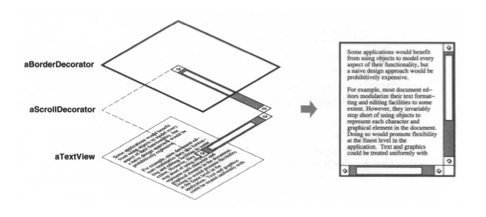
\includegraphics[height=1.75in]{gof-decorator-diagram.png}
\end{center}



\end{frame}
%------------------------------------------------------------------------

%------------------------------------------------------------------------
\begin{frame}[fragile]{{\tt JScrollPane} and the Decorator Pattern}


The Swing l ibrary provides a scrollbar decorator called {\tt JScrollPane}.  Using it is easy:
\begin{lstlisting}[language=Java]
add(new JScrollPane(new JList(employeeListModel)), BorderLayout.CENTER);
\end{lstlisting}
By simply wrapping our {\tt JList} in a {\tt JScrollPane} the list will show horizontal and vertical scroll bars as needed.

\begin{center}
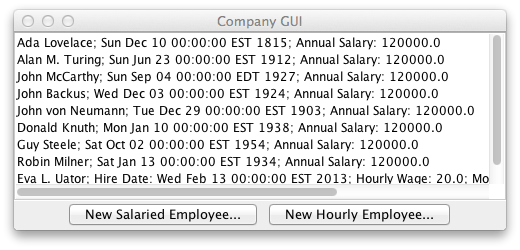
\includegraphics[height=1.75in]{CompanyGui.png}
\end{center}


\end{frame}
%------------------------------------------------------------------------

%------------------------------------------------------------------------
\begin{frame}[fragile]{Custom Dialogs with {\tt JDialog}}


To create a custom dialog, extend {\tt JDialog}.  Custom dialogs require consideration of

\begin{itemize}
\item Modality - should the dialog be modal or modeless?
\item Visual design - a dialog box is a visual component just like any other GUI component.
\item UI design:
\begin{itemize}
\item Make it clear how the dialog box fits into the overall GUI application (how it is launched, what happens if the user clicks OK or Cancel).
\item Make it clear what the user is expected to do with the dialog.
\item Give the user useful error messages if they do something wrong.
\end{itemize}
\end{itemize}

look at some examples in the \link{\code/swing/companygui/}{Company GUI} (particularly \link{\code/swing/companygui/src/edu/gatech/cs1331/companygui/SalariedEmployeeDialog.java}{SalariedEmployeeDialog.java} and \link{\code/swing/companygui/src/edu/gatech/cs1331/companygui/HourlyEmployeeDialog.java}{HourlyEmployeeDialog.java}.

\end{frame}
%------------------------------------------------------------------------


%------------------------------------------------------------------------
\begin{frame}[fragile]{Programming Exercise: Word Count GUI}

Write a simple GUI for the word count program we wrote a few days ago.
\begin{itemize}
\item Write a main class that uses a {\tt JFileChooser} to select the file.
\begin{itemize}
\item Read the API docs and figure out how to restrict the {\tt JFileChooser} to show only text files.
\end{itemize}
\item Update your {\tt WordCount} class so that it's a class that takes a file in the constructor, and has a single method {\tt getWordCounts()} that returns a {\tt Map<String, Integer>} that maps from words to their counts.
\begin{itemize}
\item Bonus: make your {\tt WordCount} class {\tt Iterable}.
\end{itemize}

\item Display the word counts in a {\tt JList} with scroll bars.
\begin{itemize}
\item Even better: use a {\tt JTable} to display the words and associated counts.
\end{itemize}
\item Include a single button at the bottom of your application's main frame that exits the program when clicked.
\end{itemize}


\end{frame}
%------------------------------------------------------------------------

% %------------------------------------------------------------------------
% \begin{frame}[fragile]{}


% \begin{lstlisting}[language=Java]

% \end{lstlisting}

% \begin{itemize}
% \item
% \end{itemize}


% \end{frame}
% %------------------------------------------------------------------------


\end{document}
